\subsection{Architektur}

\subsection{Domain Model}

\begin{figure}[H]
\centering
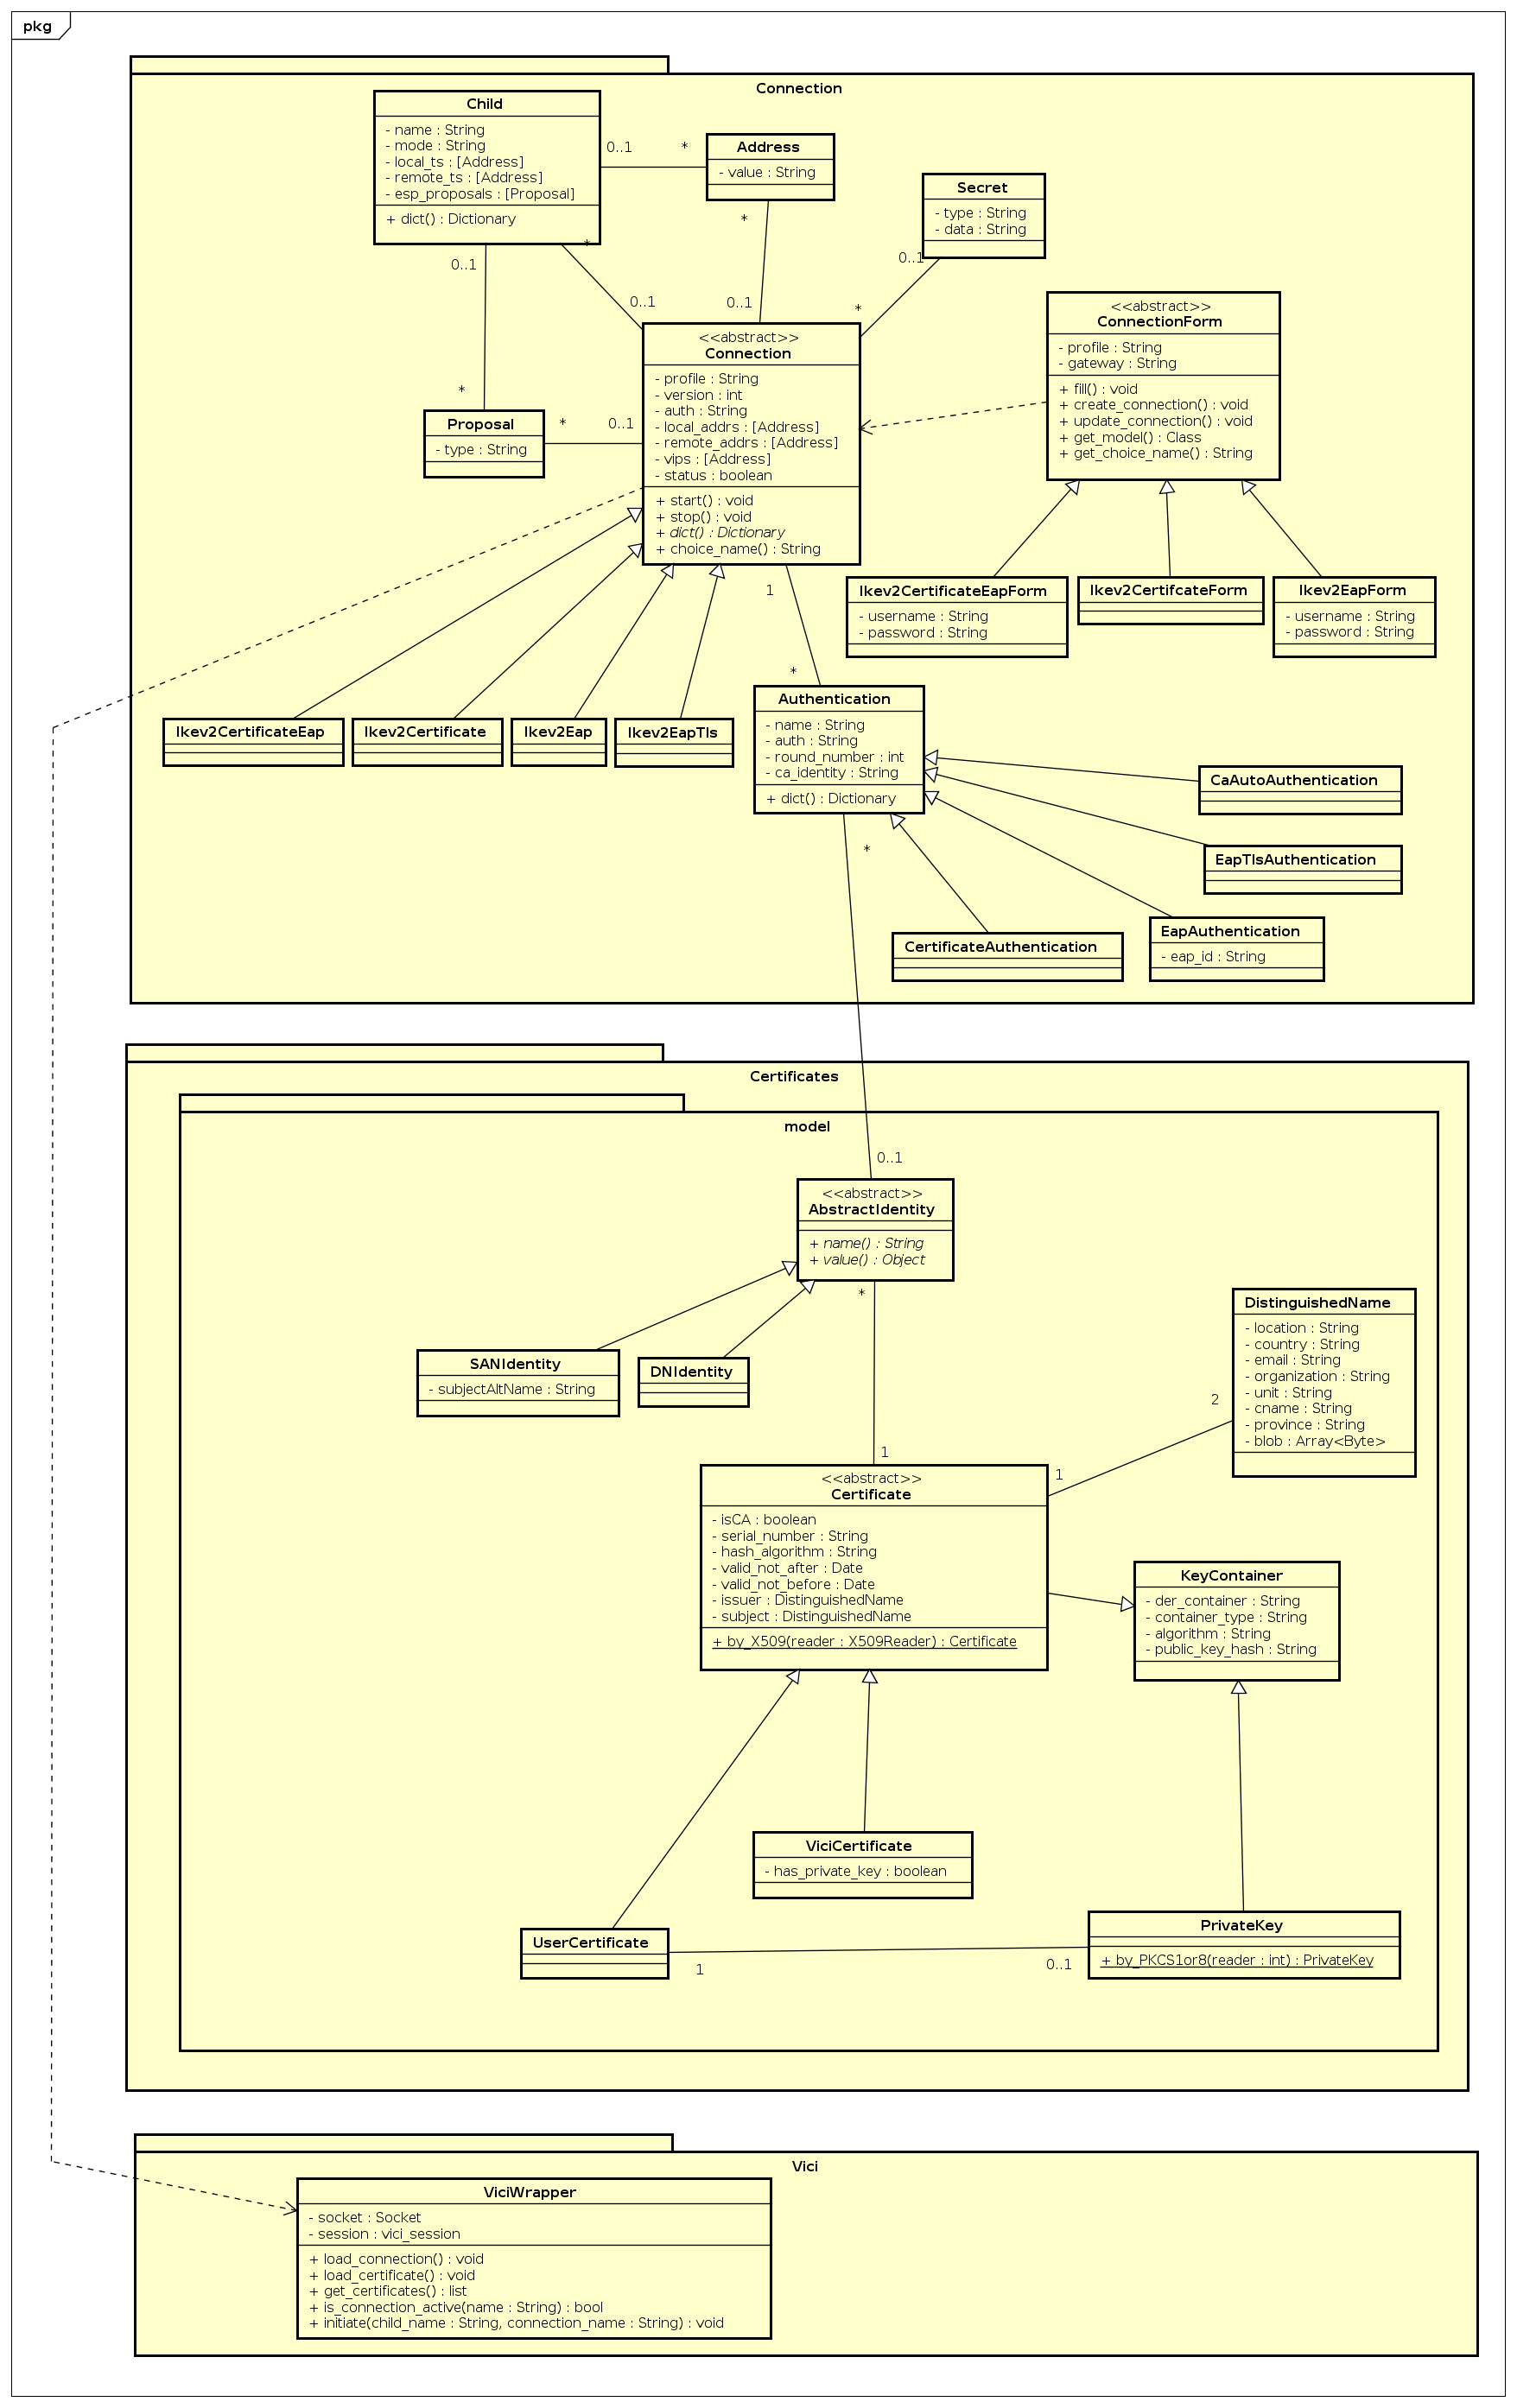
\includegraphics[width=420pt]{images/domain_model_strongman.png}
\caption[Domain Model]{Domain Model}
\end{figure}

Das Domain Model soll im Allgemeinen eine Abstraktion der Vici-Schnittstelle darstellen.
Dabei ist die Connection Klasse zentral. Damit die verschiedenen Authentisierungsmethoden unterstütz werden können, wird von Connection geerbt.

Weiter sind die Certificates ein essentieller Bestandteil, diese sind über die Hilfsklasse AbstractIdentity mit der Authentication verbunden, welche wiederum ein Verbindung zur Connection hat.

\newpage